%# -*- coding: utf-8-unix -*-
% !TEX program = xelatex
% !TEX root = ../thesis.tex
% !TEX encoding = UTF-8 Unicode
%%==================================================
%% chapter01.tex for SJTU Master Thesis
%%==================================================

%\bibliographystyle{sjtu2}%[此处用于每章都生产参考文献]


\chapter{控制器}
\label{chap:chapter02}
船舶系统按不同的推进器配置可分为欠驱动(Underactuated systems)和全驱动(fully-actuated
systems)系统。通常所说的动力定位船舶或者平台即为全驱动系统,这类系统的输入量不少于控制量。
而欠驱动船舶是输入比要控制的量少的一类典型系统。
本章介绍船舶控制器,主要包括PID控制器,轨迹跟踪算法和推力分配算法。

\section{推力分配}
\subsection{推进器简介}
船用推进器主要包括隧道式螺旋桨、全回转螺旋桨、固定式螺旋桨加舵以及泵推。其简图如\ref{fig:thrustertype}

\begin{figure}[!htp]
  \centering
  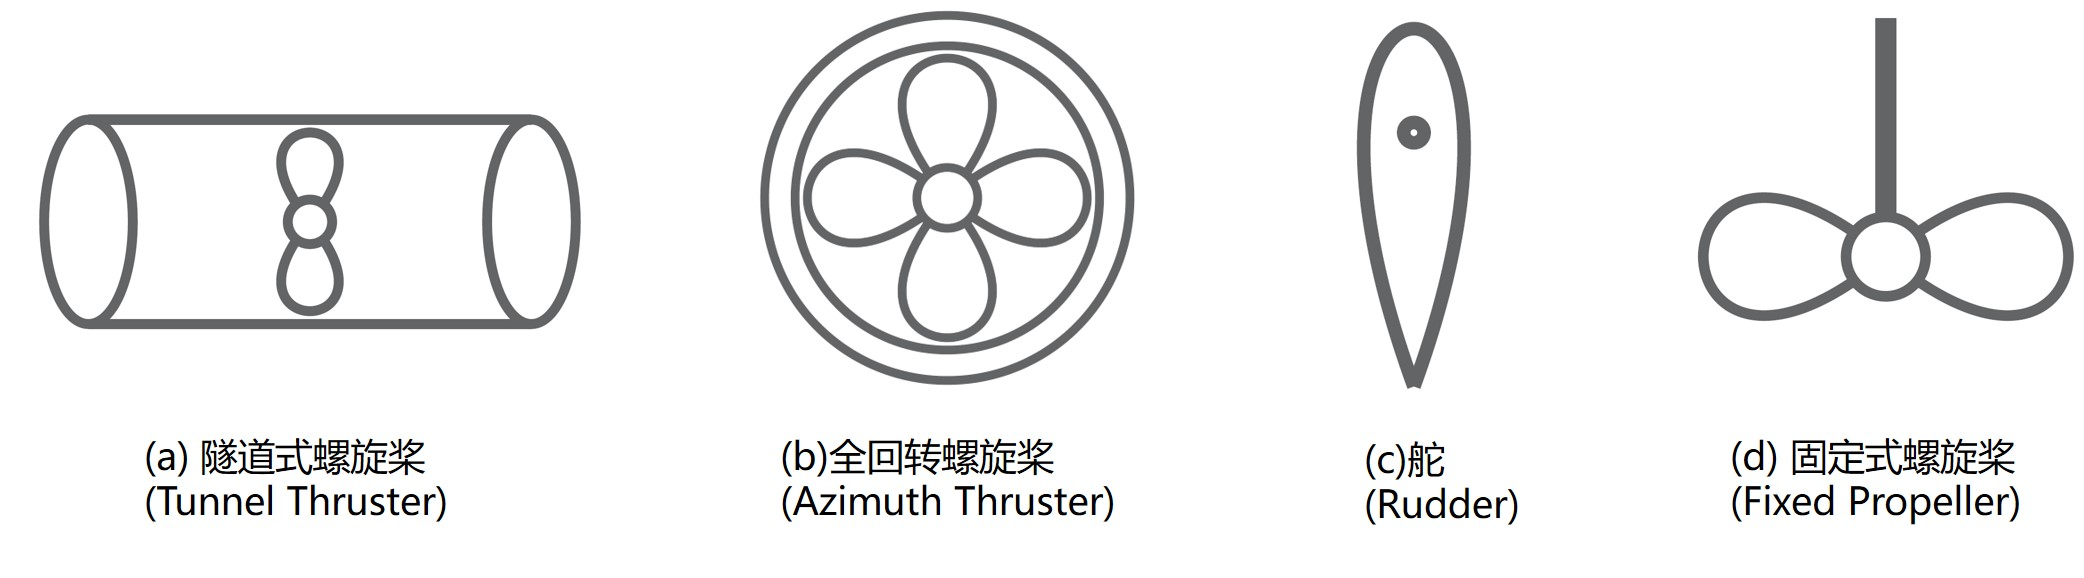
\includegraphics[width=15cm]{chapter02/thrustertype.jpg}
  \bicaption[常见船舶推进器示意图]
    {常见船舶推进器示意图}
    {Sketch of common thrusters of vessel}
  \label{fig:thrustertype}
\end{figure}

对于每种推进器,其推力可根据船级社DNVGL的规范 \cite{DNVGL2016DP}估算得到。
\begin{equation}
  \label{eq:effectivethrust}
    {\tau}_{e} = \beta_T {\tau}_{n}
\end{equation}
其中,${\tau}_{e}$称为有效推力,${\tau}_{n}$是名义推力,$\beta_T$是
推力损失系数。
\begin{equation}
  \label{eq:nominalthrust}
    {\tau}_{n} = \eta_1 \eta_2 \left(D\times P\right)^{\frac{2}{3}}
\end{equation}
其中,$D$是以米(m)为单位的螺旋桨直径,$P$是以千瓦(kW)为单位的推进器功率。$\eta_1$和
$\eta_2$的取值参见DNVGL的规范。

对于舵,其推力
\begin{equation}
  \begin{aligned}
  \label{eq:rudderthrust}
    {\tau}_{surge} &= {\tau}_e (1-C_x \alpha^2) \\
    {\tau}_{sway} &= {\tau}_e C_y \alpha \\
    C_x &= 0.02 C_y  \\
    C_y &= 0.0126 k_1 k_2 \frac{A_r}{D^2}
  \end{aligned}
\end{equation}
其中$\alpha$是以度$(^{\circ})$为单位的舵角,一般舵角不会超过$30^{\circ}$。
$A_r$是舵可转动部分的面积。$k_1$和$k_2$的取值参见规范。

\subsection{推力分配模型}
推力分配算法将广义力作为输入,通过建模并优化得到每个推进器上的转速和推力。

\begin{figure}[!htp]
  \centering
  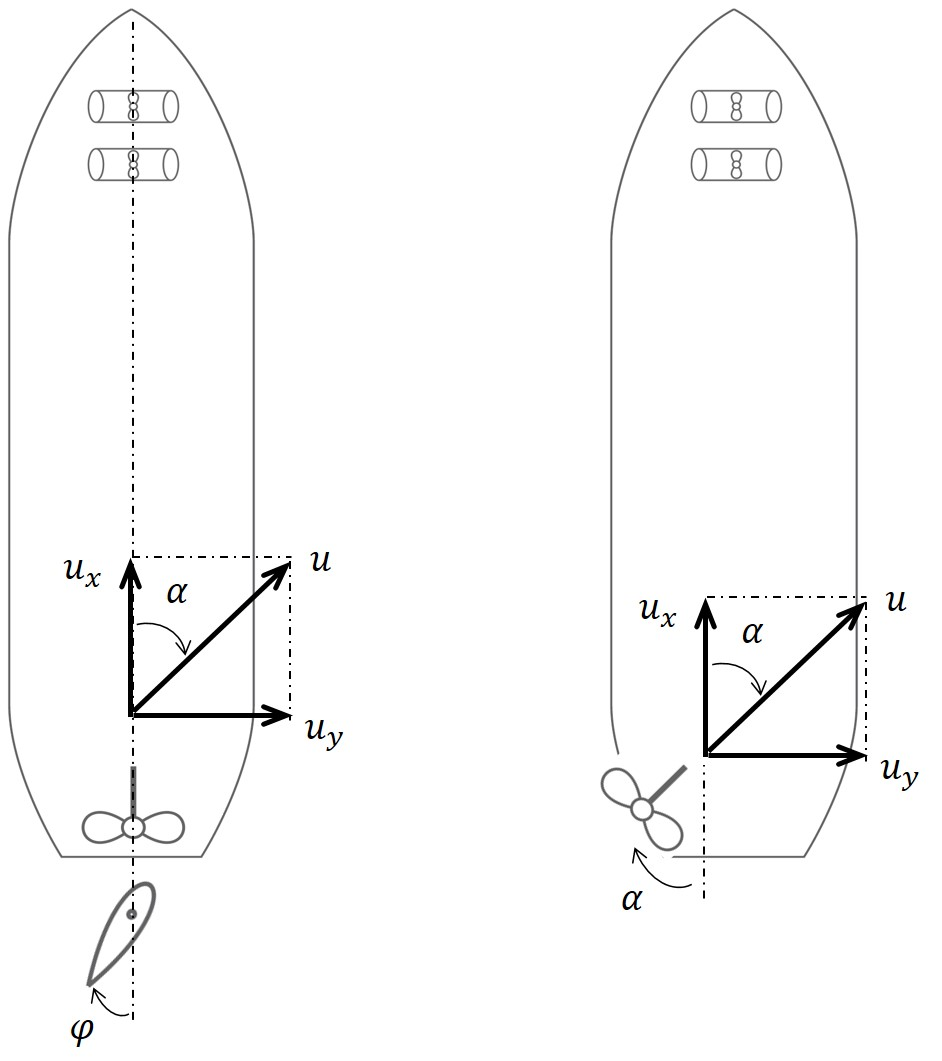
\includegraphics[width=10cm]{chapter02/thrusteralpha.jpg}
  \bicaption[螺旋桨角度的定义]
    {螺旋桨角度的定义}
    {Sketch of azimuth of each thruster}
  \label{fig:thrusteralpha}
\end{figure}


\begin{equation}
  \label{eq:eachthruster}
    {\bm{\tau}}(t) = \bm{B}(\bm{\alpha} )  \cdot \bm{u}
\end{equation}
其中,$\bm{u}=[u_1,u_2, \dots, u_m]^T \in \mathbb{R}^m$ 代表每个推进器产生的推力,
$\bm{\alpha}=[\alpha_1, \alpha_2, \dots, \alpha_m ]^T \in \mathbb{R}^m$ 代表
每个推进器的角度,其定义参见图\ref{fig:thrusteralpha}。
假设在随体坐标系中,推进器相对于重心的位置为$(l_{xi},l_{yi})$, 则矩阵
$\bm{B}(\bm{\alpha} ) \in \mathbb{R}^{3 \times m}$可得
\begin{equation}
  \label{eq:Balpha}
\bm{B}(\bm{\alpha})=\left[\begin{array}{cccc}{
\cos \alpha_{1}} & {\cos \alpha_{2}} & \cdots & {\cos \alpha_{m}} \\
{\sin \alpha_{1}} & {\sin \alpha_{2}}  & \cdots & {\sin \alpha_{m}} \\
{l_{x 1} \sin \alpha_{1}-l_{y 1} \cos \alpha_{1}} &
{l_{x 2} \sin \alpha_{2}-l_{y 2} \cos \alpha_{2}} &
\cdots  &
{l_{x m} \sin \alpha_{m}-l_{y m} \cos \alpha_{m}}\end{array}\right]
\end{equation}

我们假设推力和螺旋桨转速$n$呈二次关系
\begin{equation}
  \label{eq:thrustrotation}
    u_i= K_i n_i |n_i|
\end{equation}
其中,$K_i$可以从推力测量实验(详见\ref{sec:parameters}节)得到。

我们将推力分配问题转化为带有线性约束的二次规划问题(Quadratic Programming)
\cite{johansen2004constrained}, 目前我们采用Mosek或osqp求解器来计算优化解。
\begin{equation}
  \label{eq:qpmin}
    \begin{aligned}
      \min J(\Delta \bm{\alpha}, \Delta \bm{u}, \bm{s})
      &= \sum_{i=1}^{m} \left(
      \frac{\mathrm{d} W_{i}}{\mathrm{d} u_{i}}\left( u_{0, i} \right)
      \Delta u_{i}+
      \frac{\mathrm{d}^{2} W_{i}}{\mathrm{d} u_{i}^{2}}\left(u_{0, i}\right)
      \Delta u_{i}^{2} \right)+
      \Delta \bm{\alpha}^{T} \bm{\Omega} \Delta \bm{\alpha}+\bm{s}^{T} \bm{Q} \bm{s} \\
      &+\frac{\mathrm{d}}{\mathrm{d}\alpha}\left(\frac{\rho}{\varepsilon+
      \operatorname{det}\left(\bm{B}(\bm{\alpha})\bm{B}^{T}(\bm{\alpha})\right)}\right)
      _{\alpha=\alpha_{0}} \cdot \Delta \bm{\alpha} \\
      &=\bm{g}_{\Delta u}^{T} \cdot \Delta \bm{u}+\Delta \bm{u}^{T} \bm{Q}_{\Delta u}
      \Delta \bm{u}+\bm{s}^{T} \bm{Q} \bm{s}+\Delta \bm{\alpha}^{T}
      \bm{\Omega} \Delta \bm{\alpha}+\bm{d}_{\rho}^{T} \Delta \bm{\alpha}
    \end{aligned}
\end{equation}

\begin{equation}
  \label{eq:qpconstraints}
    \begin{aligned}
      \text{subject to } \\
      &\bm{s}+\bm{B}\left(\bm{\alpha}_{0}\right) \cdot \Delta \bm{u}+
      \frac{\partial}{\partial \bm{\alpha}}(\bm{B}(\bm{\alpha}) \bm{u})
      _{\bm{\alpha}=\bm{\alpha_{0}}} \cdot \Delta \bm{\alpha}
      =\bm{\tau}-\bm{B}\left(\bm{\alpha}_{0}\right) \cdot \bm{u}_{0} \\
      &\underline{\Delta \bm{u}} \leq \Delta \bm{u} \leq \overline{\Delta \bm{u}}
      \\ &\underline{\Delta \bm{\alpha}} \leq \Delta \bm{\alpha} \leq \overline{\Delta \bm{\alpha}}
    \end{aligned}
\end{equation}
这里,$\leq$代表向量不等式,$W$代表推进器的功率,通常假设$W=u^{\frac{3}{2}}$。
 $u_{0,i}$代表上一时刻第$i$个推进器产生的推力,$s$代表
估计推力与预期推力的偏差。我们用$\bm{z}=[\Delta \bm{u}, \Delta \bm{\alpha},
\bm{s}]^T \in \mathbb{R}^{2m+3}$,上述方程简化可得
\begin{equation}
  \label{eq:qpsimple}
  \begin{aligned}
  & \min \bm{z}^{T} \bm{H} \bm{z}+\bm{g}^{T} \bm{z} \\
  &\text { s.t. }  \bm{P z} \leq \bm{h} \\
  &\qquad \bm{c z}=\bm{b}
  \end{aligned}
\end{equation}

\begin{equation}
  \label{eq:qpsimple1}
  \begin{aligned}
    & \bm{c}=
    \begin{bmatrix}
      \bm{B}\left(\bm{\alpha}_0 \right)  
      & \frac{\partial}{\partial \bm{\alpha}} \left( \bm{B}(\bm{\alpha})
      \bm{u} \right) |_{\bm{u}=\bm{u}_{0}, \bm{\alpha}=\bm{\alpha}_{0}}
      & \bm{I}
    \end{bmatrix} \\
    & \bm{b}=
    \bm{\tau}-  \bm{B} ( \bm{\alpha_0} ) \cdot \bm{u_0} \\
    & \bm{H}=
    \begin{bmatrix}
      \bm{Q}_{\Delta \bm{u}} & \bm{0} & \bm{0} \\
      \bm{0} & \bm{\Omega} & \bm{0} \\
      \bm{0} & \bm{0} & \bm{Q}
    \end{bmatrix} \\
    & \bm{g}=
    \begin{bmatrix}
       \bm{g}_{\Delta \bm{u}} \\
       \bm{d}_{\rho} \\
       \bm{0}
    \end{bmatrix} \\
    & \bm{P}=
    \begin{bmatrix}
       \bm{I} & \bm{0} & \bm{0} \\
       \bm{-I} & \bm{0} & \bm{0} \\
       \bm{0} & \bm{I} & \bm{0} \\
       \bm{0} & \bm{-I} & \bm{0} \\
    \end{bmatrix} \\
    & \bm{h}=
    \begin{bmatrix}
       \overline{\Delta \bm{u}} \\
       -\underline{\Delta \bm{u}}  \\
       \overline{\Delta \bm{\alpha}} \\
       -\underline{\Delta \bm{\alpha}}
    \end{bmatrix}
  \end{aligned}
\end{equation}

\begin{equation}
  \label{eq:qpsimple2}
  \begin{aligned}
    &\bm{g}_{\Delta \bm{u}}=
    \begin{bmatrix}
      \frac{3}{2} u_{0,1}^{\frac{1}{2}} \\
      \frac{3}{2} u_{0,2}^{\frac{1}{2}} \\
      \vdots \\
      \frac{3}{2} u_{0, m}^{\frac{1}{2}}
    \end{bmatrix} \\
    & \bm{Q}_{\Delta \bm{u}} =
    \begin{bmatrix}
      \frac{3}{4} u_{0,1}^{-\frac{1}{2}} & & & \\
      & \frac{3}{4} u_{0,2}^{-\frac{1}{2}} & & \\
      & & \ddots & \\
      & & & \frac{3}{4} u_{0,m}^{-\frac{1}{2}}
    \end{bmatrix} \\
  \end{aligned}
\end{equation}


每个推进器的推力变化和角度变化的上下限是实时变化的,针对每种推进器
,其约束条件将在下面几小节讨论。


\subsection{求解器}
目前我们采用Mosek或osqp求解器来计算优化解,由于Mosek是商业求解器,之后会逐渐采用开源的求解器来替代Mosek。

\subsubsection{Mosek}
本节介绍使用Mosek求解器的一些细节。我们用$m$表示推进器的数量,$n$表示推力的维度($n=3$),则优化问题(\ref{eq:qpsimple})中的参数
$ \bm{z} \in \mathbb{R}^{2 m + n} , \, \bm{b} \in \mathbb{R}^{n} , \, \bm{c} \in 
\mathbb{R}^{{n}\times (2m+n)}$

\begin{itemize}
  \item 变量$ \bm{z}$的约束 (对应$\bm{Pz \leq h}$),如表(\ref{tab:mosekvariablebound})

  \item 线性约束 (对应$\bm{cz = b}$), 如表(\ref{tab:moseklinearconstraint})

  \item 目标函数(对应$\bm{z}^{T} \bm{H} \bm{z}+\bm{g}^{T} \bm{z}$),如表(\ref{tab:mosekobjective})
\end{itemize}

\begin{table}[htbp]
  \caption{Mosek中变量约束(RT代表实时变化量)}
  \centering
  \begin{tabular}{@{}lllll@{}}
    \toprule
    \multirow{2}{*}{Type} & \multirow{2}{*}{Name} & \multicolumn{3}{c}{Index}               \\ \cmidrule(l){3-5} &               & 0:(m-1)               & m:(2m-1)    & 2m:(2m+n-1) \\ \cmidrule(r){1-2}
    MSKboundeye           & bkx{[}{]}             & MSK\_BK\_RA & MSK\_BK\_RA & MSK\_BK\_FR \\
    double                & blx{[}{]}             & RT   & RT    & -MSK\_INFI  \\
    double                & bux{[}{]}             & RT   & RT    & MSK\_INFI   \\ \bottomrule
    \end{tabular}
  \label{tab:mosekvariablebound}
\end{table}

\begin{table}[htbp]
  \caption{Mosek中线性约束(RT代表实时变化量)}
  \centering
  \begin{tabular}{@{}llllllllll@{}}
  \toprule
  \multirow{2}{*}{Type} & \multirow{2}{*}{Name} & \multicolumn{8}{l}{Index}   \\ \cmidrule(l){3-10} 
                        &    & 0  & 1  & 2   & ... & 2m-1  & 2m   & 2m+1 & 2m+2 \\ \cmidrule(r){1-2}
  MSKint32t & aptrb{[}{]}  & 0   & 3         & 6         & ... & 6m-3      & 6m   & 6m+1 & 6m+2 \\
  MSKint32t & aptre{[}{]}  & 3   & 6         & 9         & ... & 6m        & 6m+1 & 6m+2 & 6m+3 \\
 \bottomrule
  \end{tabular}

  \begin{tabular}{@{}lllllllllllllll@{}}
  \toprule
  \multirow{2}{*}{Type} & \multirow{2}{*}{Name} & \multicolumn{13}{l}{Index}    \\ \cmidrule(l){3-15} 
  &   & 0  & 1  & 2  & 3  & 4  & 5  & ... & 6m-3 & 6m-2 & 6m-1 & 6m & 6m+1 & 6m+2 \\ \cmidrule(r){1-2}
  MSKint32t  & asub{[}{]}   & 0  & 1  & 2  & 0  & 1  & 2  & ... & 0    & 1    & 2    & 0  & 1    & 2    \\
  double     & aval{[}{]}   & RT & RT & RT & RT & RT & RT & ... & RT   & RT   & RT   & 1  & 1    & 1    \\ \bottomrule
  \end{tabular}

  \begin{tabular}{@{}lllll@{}}
  \toprule
  \multirow{2}{*}{Type} & \multirow{2}{*}{Name} & \multicolumn{3}{l}{Index}      \\ \cmidrule(l){3-5} 
                        &               & 0           & 1           & 2           \\ \cmidrule(r){1-2}
  MSKboundkeye          & bkc{[}{]}             & MSK\_BK\_FX & MSK\_BK\_FX & MSK\_BK\_FX \\
  double                & blc{[}{]}             & RT          & RT          & RT          \\
  double                & buc{[}{]}             & blc{[}0{]}  & blc{[}1{]}  & blc{[}2{]}  \\ \bottomrule
  \end{tabular}

  \label{tab:moseklinearconstraint}
\end{table}

\begin{table}[htbp]
  \caption{Mosek中目标函数(RT代表实时变化量)}
  \centering
  \begin{tabular}{@{}llllllllllll@{}}
  \toprule
  \multirow{2}{*}{Type} & \multirow{2}{*}{Name} & \multicolumn{10}{l}{Index}     \\ \cmidrule(l){3-12} 
                &  & 0  & 1  & ... & m-1 & m     & ... & 2m-1 & 2m & 2m+1 & 2m+2 \\ \cmidrule(r){1-2}
  MSKint32t   & qsubi{[}{]}    & 0  & 1  & ... & m-1 & m     & ... & 2m-1 & 2m & 2m+1 & 2m+2 \\
  MSKint32t   & qsubj{[}{]}    & 0  & 1  & ... & m-1 & m     & ... & 2m-1 & 2m & 2m+1 & 2m+2 \\
  double      & qval{[}{]}     & RT & RT & ... & RT  & $\bm{\Omega}[0][0]$ & ... &  $\bm{\Omega}[m-1][m-1]$    &  $\bm{Q}[0][0]$  &  $\bm{Q}[1][1]$  & $\bm{Q}[2][2]$  \\ 
  \bottomrule
  \end{tabular}
  \label{tab:mosekobjective}
\end{table}


\subsubsection{osqp}
osqp是由牛津大学和斯坦福大学合作开发的一款二次规划求解器。


\subsection{欠驱动}
目前大部分船舶是欠驱动的,常见的欠驱动船舶的推进器配置有:(1) 双固定式尾推; (2) 主推配合
船舵
\subsubsection{双固定式尾推}
\begin{itemize}
	\item 转向可通过两个螺旋桨差速实现
	\item 通常用伺服电机或者步进电机带动螺旋桨
	\item 对于步进电机,为了防止过快的正反转切换,我们人为限制其切换速度。
\end{itemize}

推力曲线如\ref{fig:twinfixed}所示,正向的推力常数为$k^+$, 负向的为$k^-$。我们用$v_n$
表示螺旋桨转速的最大变化率,$\Delta t$表示采样时间,$t_{p2n}$表示螺旋桨从正到负或者从负到
正的切换时间

\begin{equation}
  \begin{aligned}
    & \Delta n_{max} = v_n \Delta t \\
    & \Delta n_{max}^{p2n} = \frac{2 \Delta n_{max} \Delta t}{t_{p2n}}
  \end{aligned}
\end{equation}

为了考虑正反转切换时间,我们采用了两种不同的转速限制:通常转速变化的极值为$\Delta n_{max}$;
而在$-\Delta n_{max}$和$\Delta n_{max}$之间,转速变化的极值为$\Delta n_{max}^{p2n} $,
进而我们可以得到不同转速下,优化问题的约束条件。

\begin{enumerate}
  \item $n_0 \geq \Delta n_{max}$
  \begin{itemize}
    \item $\underline{\Delta \alpha} = \overline{\Delta \alpha} = 0$
    \item $\overline{\Delta u}= \min \left( u_{max}-k^+ n_0^2 \, , \,
    k^+ (n_0+ \Delta n_{max})^2 - k^+ n_0^2 \right)$
    \item $\underline{\Delta u}=k^+ (n_0 - \Delta n_{max})^2 - k^+ n_0^2 $
  \end{itemize}

  \item $\Delta n_{max}^{p2n} \leq n_0 < \Delta n_{max}$
  \begin{itemize}
    \item $\underline{\Delta \alpha} = \overline{\Delta \alpha} = 0$
    \item $\overline{\Delta u}= k^+ (n_0 + \Delta n_{max}^{p2n})^2 - k^+ n_0^2$
    \item $\underline{\Delta u}=k^+ (n_0 - \Delta n_{max}^{p2n})^2 - k^+ n_0^2 $
  \end{itemize}

  \item $0 < n_0 < \Delta n_{max}^{p2n}$
  \begin{itemize}
    \item if $u_d < 0$
    \begin{itemize}
      \item $\underline{\Delta \alpha} = \overline{\Delta \alpha} = \pi$
      \item $\overline{\Delta u}= \underline{\Delta u}=
      k^- (n_0 - \Delta n_{max}^{p2n})^2 - k^+ n_0^2$
    \end{itemize}
    \item elseif $u_d \geq 0$
    \begin{itemize}
      \item $\underline{\Delta \alpha} = \overline{\Delta \alpha} = 0$
      \item $\overline{\Delta u}= \underline{\Delta u}=
      k^+ (n_0 + \Delta n_{max}^{p2n})^2 - k^+ n_0^2$
    \end{itemize}
  \end{itemize}

  \item $-\Delta n_{max}^{p2n} < n_0 < 0$
  \begin{itemize}
    \item if $u_d > 0$
    \begin{itemize}
      \item $\underline{\Delta \alpha} = \overline{\Delta \alpha} = -\pi$
      \item $\overline{\Delta u}= \underline{\Delta u}=
      k^+ (n_0 + \Delta n_{max}^{p2n})^2 - k^- n_0^2$
    \end{itemize}
    \item elseif $u_d \leq 0$
    \begin{itemize}
      \item $\underline{\Delta \alpha} = \overline{\Delta \alpha} = 0$
      \item $\overline{\Delta u}= \underline{\Delta u}=
      k^- (n_0 - \Delta n_{max}^{p2n})^2 - k^- n_0^2$
    \end{itemize}
  \end{itemize}

  \item $-\Delta n_{max} < n_0 \leq -\Delta n_{max}^{p2n} $
  \begin{itemize}
    \item $\underline{\Delta \alpha} = \overline{\Delta \alpha} = 0$
    \item $\overline{\Delta u}= k^- (n_0 - \Delta n_{max}^{p2n})^2 - k^- n_0^2$
    \item $\underline{\Delta u}=k^- (n_0 + \Delta n_{max}^{p2n})^2 - k^- n_0^2 $
  \end{itemize}

  \item $n_0 \leq -\Delta n_{max}$
  \begin{itemize}
    \item $\underline{\Delta \alpha} = \overline{\Delta \alpha} = 0$
    \item $\overline{\Delta u}= \min \left( u_{min}-k^- n_0^2 \, , \,
    k^- (n_0 - \Delta n_{max})^2 - k^- n_0^2 \right)$
    \item $\underline{\Delta u}=k^- (n_0 + \Delta n_{max})^2 - k^- n_0^2 $
  \end{itemize}
\end{enumerate}

其中,$ u_d $表示每个推进器上期望的推力,如图\ref{fig:twinfixed1}所示,
\begin{equation}
  \begin{aligned}
    &u_1 = \frac{\tau_x}{2} + \frac{\tau_M}{2 l} \\
    &u_2 = \frac{\tau_x}{2} - \frac{\tau_M}{2 l} \\
  \end{aligned}
\end{equation}

\begin{figure}[!htp]
  \centering
  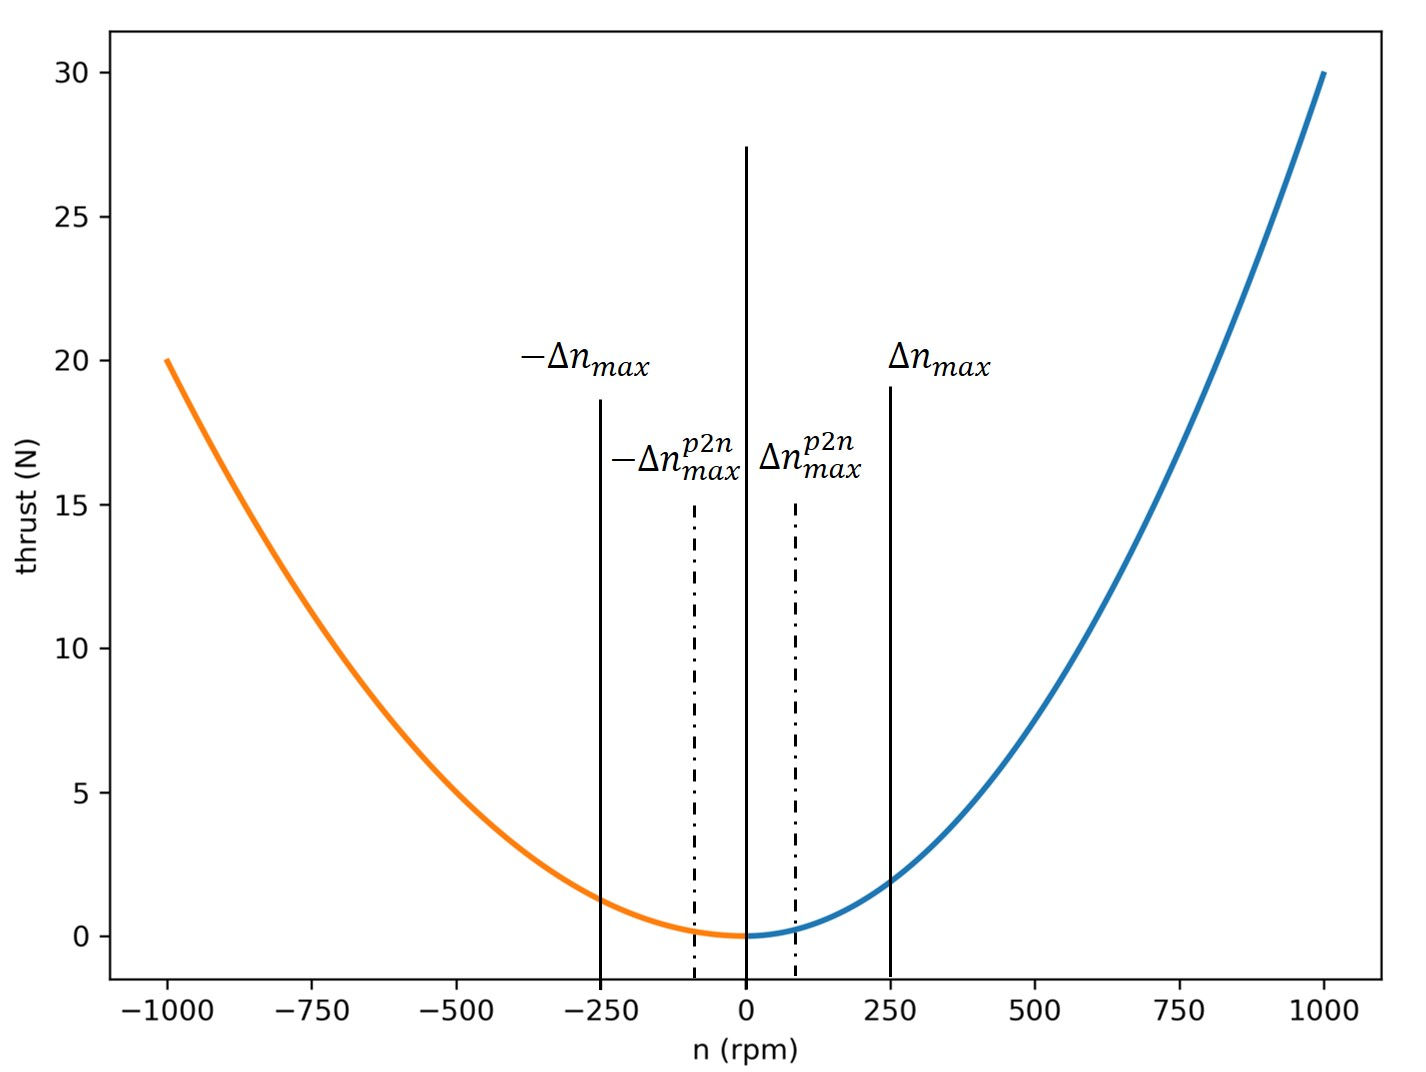
\includegraphics[width=10cm]{chapter02/twinfixed.jpg}
  \bicaption[固定式双尾推螺旋桨的推力曲线]
    {固定式双尾推螺旋桨的推力曲线}
    {Thrust(N) vs. rotational speed (rpm) of Twin fixed thruster}
  \label{fig:twinfixed}
\end{figure}

\begin{figure}[!htp]
  \centering
  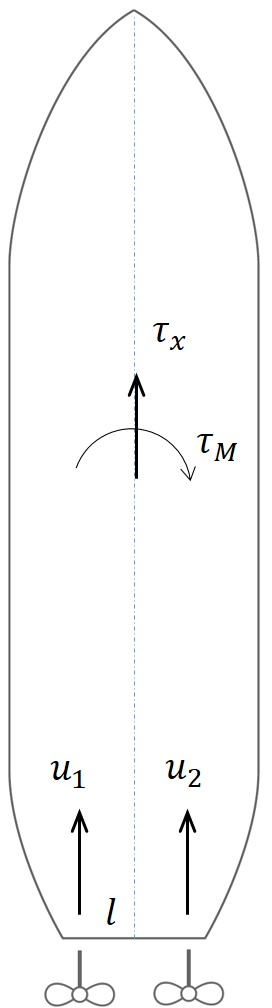
\includegraphics[width=3cm]{chapter02/twinfixed1.jpg}
  \bicaption[固定式双尾推螺旋桨的推力分配]
    {固定式双尾推螺旋桨的推力分配}
    {Thrust allocation of Twin fixed thruster}
  \label{fig:twinfixed1}
\end{figure}

\subsubsection{主推配合船舵}
如图\ref{fig:thrusteralpha}所示,船舵的舵角$\varphi$和其产生推力方向$\alpha$不一致,
他们的关系参见公式(\ref{eq:rudderthrust})。
\begin{equation}
  \begin{aligned}
    &u_x = k n^2 (1- 0.02 C_y \varphi^2) \\
    &u_y = k n^2 C_y \varphi
  \end{aligned}
\end{equation}
由此可得
\begin{equation}
  \begin{aligned}
    &\tan \alpha = \frac{C_y \varphi}{1- 0.02 C_y \varphi^2},  \quad \alpha \in
    [-\frac{\pi}{2}, \, \frac{\pi}{2}] \\
    &u=kn^2 \sqrt{(0.02C_y\varphi^2)^2+(C_y^2 -0.04 C_y)\varphi^2 +1}
  \end{aligned}
\end{equation}
利用$\tan \alpha$的单调性,我们能够计算$\alpha$的约束条件;同时,$u$的极值也可以分别计算
$kn^2$和$(0.02C_y\varphi^2)^2+(C_y^2 -0.04 C_y)\varphi^2 +1$的极值得到。

\subsection{全驱动船}
北东地(North-East-Down: NED)坐标系$\NEDframe=(x_n, y_n, z_n)$是
常用的导航坐标系,通常定义在地球表面的切平面上,其中$x$轴指向地球北,$y$轴指向地球东,
$z$轴垂直于地球表面并指向下。通常对于海上船舶,经纬度的变化并不大,我们可以假定$\NEDframe$
是惯性参考系。

\subsubsection{隧道式艏侧推}
\begin{enumerate}
  \item $n_0 \geq \Delta n_{max}$
  \begin{itemize}
    \item $\underline{\Delta \alpha} = \overline{\Delta \alpha} = 0$
    \item $\overline{\Delta u}= \min \left( u_{max}-k^+ n_0^2 \, , \,
    k^+ (n_0+ \Delta n_{max})^2 - k^+ n_0^2 \right)$
    \item $\underline{\Delta u}=k^+ (n_0 - \Delta n_{max})^2 - k^+ n_0^2 $
  \end{itemize}

  \item $0 < n_0 < \Delta n_{max}$
  \begin{itemize}
    \item if $u_d < 0$
    \begin{itemize}
      \item $\underline{\Delta \alpha} = \overline{\Delta \alpha} = -\pi$
      \item $\overline{\Delta u}= \underline{\Delta u}=
      k^- (n_0 - \Delta n_{max})^2 - k^+ n_0^2$
    \end{itemize}
    \item elseif $u_d \geq 0$
    \begin{itemize}
      \item $\underline{\Delta \alpha} = \overline{\Delta \alpha} = 0$
      \item $\overline{\Delta u}= k^+ (n_0 + \Delta n_{max})^2 - k^+ n_0^2$
      \item $\underline{\Delta u}=- k^+ n_0^2$
    \end{itemize}
  \end{itemize}

  \item $-\Delta n_{max} < n_0 < 0$
  \begin{itemize}
    \item if $u_d > 0$
    \begin{itemize}
      \item $\underline{\Delta \alpha} = \overline{\Delta \alpha} = \pi$
      \item $\overline{\Delta u}=\underline{\Delta u}=  k^+ (n_0 + \Delta n_{max})^2 - k^- n_0^2$
    \end{itemize}
    \item elseif $u_d \leq 0$
    \begin{itemize}
      \item $\underline{\Delta \alpha} = \overline{\Delta \alpha} = 0$
      \item $\overline{\Delta u}= k^- (n_0 - \Delta n_{max})^2 - k^- n_0^2$
      \item $\underline{\Delta u}=- k^- n_0^2$
    \end{itemize}
  \end{itemize}

  \item $n_0 \leq -\Delta n_{max}$
  \begin{itemize}
    \item $\underline{\Delta \alpha} = \overline{\Delta \alpha} = 0$
    \item $\overline{\Delta u}= \min \left( u_{min}-k^- n_0^2 \, , \,
    k^- (n_0 - \Delta n_{max})^2 - k^- n_0^2 \right)$
    \item $\underline{\Delta u}=k^- (n_0 + \Delta n_{max})^2 - k^- n_0^2 $
  \end{itemize}
\end{enumerate}

\section{PID控制器}
PID控制器将位置和速度误差作为输入,计算得到预期的广义力,并通过推力分配算法给出每个推进器
的转速和角度。对于一般的PID控制器,我们定义$e(t) = SP - PV$为误差, 则
\begin{equation}
    u(t)= u_{bias} + K_p e(t)+ \frac{K_I}{\tau_I} \int_0^t e(t) dt + K_d \dot{e}(t)
\end{equation}
其中,$SP$代表设定点(setpoint), $PV$代表实际点。
对于离散情况下,积分项通常为
\begin{equation}
  \sum_{i=n_t - N}^{n_t} e_i(t) \Delta t
\end{equation}
其中,$n_t$代表当前时刻,$N$表示积分长度。
一般而言,对于速度控制,我们通常采用PD控制器,可以减少超调和震荡;对于位置控制,可以用
PI控制器减少静差。

\subsection{动力定位}

\section{轨迹跟踪}

\subsection{视线跟踪法}
视线跟踪法(line of sight)\cite{fossen2003line}是一个路径规划的算法,
最早用于航空航天和导弹制导领域,其主要思路是
根据船的位置计算得到预期的首向角,从而使得船体沿着预期的路径运动。如果我们对船体的前进速度
$u$作反馈控制,即
\begin{equation}
  \lim_{t \rightarrow \infty}\left[u(t)-u_{d}(t)\right]=0
\end{equation}
其中,$u_d$是预期的前进速度。对于LOS, 我们定义$\eta = [s,\, d]^T$,则
\begin{equation}
  \begin{aligned}
      & \bm{R}(\theta_k) =
      \begin{bmatrix}
        \cos \theta_k  & \sin  \theta_k  \\
        -\sin  \theta_k & \cos \theta_k
      \end{bmatrix} \\
      & \eta =\bm{R}(\theta_k)
      \begin{bmatrix}
        x_0 - x_{wp1}\\
        y_0 - y_{wp1}
      \end{bmatrix}
  \end{aligned}
\end{equation}
\begin{equation}
  \begin{aligned}
    &\theta_{los}=\theta_r + \theta_k \\
    &\theta_k=  \arctan \frac{y_{wp2} - y_{wp1} }{ x_{wp2} - x_{wp1}} \\
    & \theta_r = \arcsin \frac{-d}{nL_{pp}}
  \end{aligned}
\end{equation}


\begin{figure}[!htp]
  \centering
  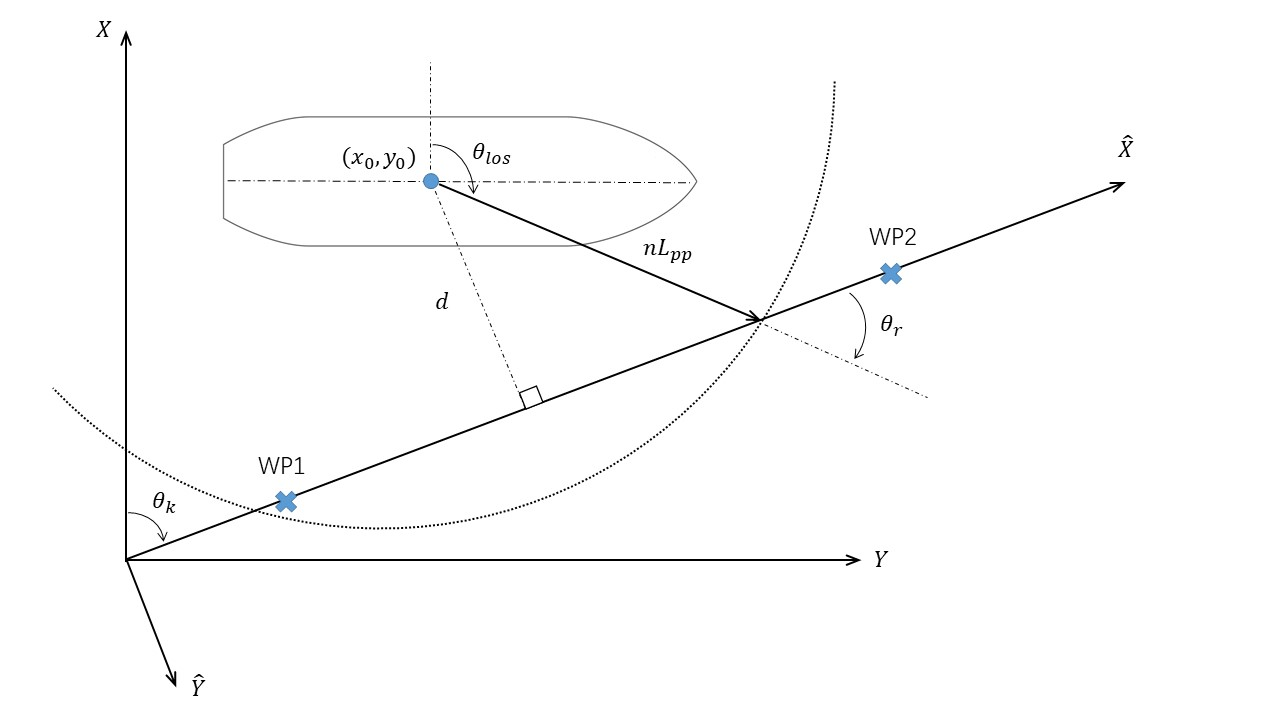
\includegraphics[width=14cm]{chapter02/los.jpg}
  \bicaption[基于视线的轨迹跟踪算法]
    {基于视线的轨迹跟踪算法}
    {Trajectory tracking using line of sight(LOS)}
  \label{fig:lineofsight}
\end{figure}




\section{参数辨识}
\label{sec:parameters}
